%  !TeX  root  =  user_guide.tex

\section{Extension Grape routier}\label{sec:roadgraph}

L'extension \toolbtntwo{plugin}{Graphe routier} est une extension C++ pour QGIS, qui calcule le chemin le plus court entre deux points sur n'importe quel polyligne et trace cde chemin au dessus le réseau routier.

\textbf{Fonctionnalités principales} :

\begin{itemize}
\item calcule le chemin, sa longueur et le temps de trajet
\item optimise par longueur ou par temps de trajet
\item export le chemin en couche vecteur
\item met en couleur les directions de la route (cela est lent et surtout utilisé pour déboguer et pour tester le paramétrage)
\end{itemize}

Vous pouvez utiliser n'importe quelle couche vecteur comme couche route dans n'importe quel format géré par QGIS. Deux lignes avec un point commun sont considérées comme connectées. Notez qu'il est obligatoire d'utiliser la projection de la couche comme projection du projet lors de l'édition de la couche route. Cela est dû au fait que le calcul de transformation des coordonnées entre différentes projections introduit 
des erreurs qui peuvent créer des discontinuités, même quand l'accrochage est utilisé.

\textbf{Dans la table attributaire de la couche, les champs suivants peuvent être utilisés} :

\begin{itemize}
\item vitesse sur la section de la route — champs numériques ;
\item direction — n'importe quel type qui peut être écrit en chaîne de caractères. Les directions avant et arrière de la géométrie correspondent à une route à sens unique, les deux directions — une route à double sens.
\end{itemize}

Si des champs n'ont pas de valeur ou n'existent pas — les valeurs par défaut sont utilisées. Vous pouvez les changer ainsi que certains paramétrages dans la fenêtre de paramétrage de l'extension.

\minisec{Usage}

Après l'activation de l'extension, vous verrez un panneau supplémentaire sur la gauche de la fenêtre principale de QGIS. Maintenant, réalisez quelques définitions dans la fenêtre \dialog{paramétrage de l'extension du graphe routier} dans le menu \mainmenuopt{Extension} \arrow \dropmenuopt{Graphe routier}. 

\begin{figure}[ht]
    \centering
    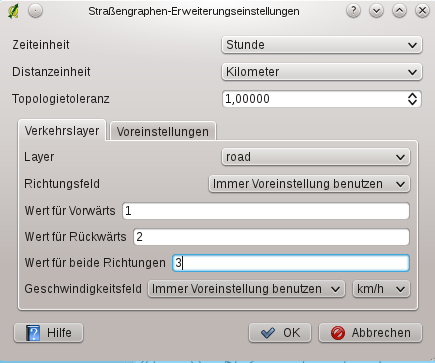
\includegraphics[clip=true, width=5cm]{roadgraph_settings}
    \caption{Définir des paramétrages pour l'extension graphe routier \nixcaption}\label{fig:roadgraphsettings}
\end{figure}

Sélectionnez un point de commencement et d'arrêt sur la couche du réseau routier et cliquez sur \button{calculer}.

\begin{figure}[ht]
    \centering
    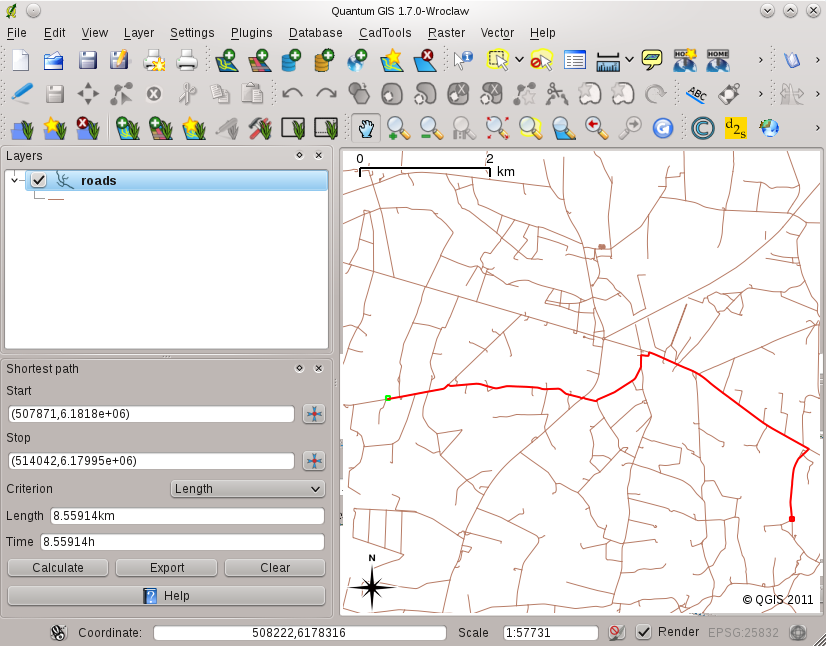
\includegraphics[clip=true, width=12cm]{roadgraph_sample}
    \caption{Extension Graphe routier \nixcaption}\label{fig:roadgraphsample}
\end{figure}

\FloatBarrier